\documentclass[11pt]{article}
\usepackage[T1]{fontenc}
\usepackage[utf8]{inputenc}
\usepackage{lmodern}
\usepackage{microtype}
\usepackage[margin=1in]{geometry}
\usepackage{amsmath,amssymb,amsthm,mathtools}
\usepackage{booktabs,array,longtable}
\usepackage{graphicx}
\usepackage[dvipsnames]{xcolor}
\usepackage{enumitem}
\usepackage{hyperref}
\usepackage[nameinlink,noabbrev]{cleveref}
\usepackage{fancyhdr}
\hypersetup{colorlinks=true,linkcolor=MidnightBlue,citecolor=MidnightBlue,
 urlcolor=MidnightBlue,pdftitle={Exact extensions of the GRH research programme},
 pdfauthor={OpenAI ChatGPT}}
\setlength{\parskip}{.25em}
\setlength{\parindent}{1.3em}
\setlength{\headheight}{14pt}
\pagestyle{fancy}
\fancyhf{}
\fancyhead[L]{\small Exact extensions of the GRH research programme}
\fancyhead[R]{\small 27 November 2026}
\fancyfoot[C]{\thepage}
\newtheorem{theorem}{Theorem}[section]
\newtheorem{lemma}[theorem]{Lemma}
\newtheorem{proposition}[theorem]{Proposition}
\newtheorem{corollary}[theorem]{Corollary}
\theoremstyle{definition}
\newtheorem{definition}[theorem]{Definition}
\newtheorem{example}[theorem]{Example}
\newtheorem{remark}[theorem]{Remark}
\newcommand{\OO}{\mathcal O}
\newcommand{\FF}{\mathbb F}
\newcommand{\RR}{\mathbb R}
\newcommand{\NN}{\mathbb N}
\newcommand{\ZZ}{\mathbb Z}
\newcommand{\Prob}{\mathbb P}
\newcommand{\EE}{\mathbb E}
\newcommand{\TV}{\operatorname{TV}}
\newcommand{\SN}{\operatorname{SN}}
\newcommand{\GL}{\operatorname{GL}}
\newcommand{\Sp}{\operatorname{Sp}}
\newcommand{\Mat}{\operatorname{Mat}}
\newcommand{\tr}{\operatorname{tr}}
\newcommand{\rank}{\operatorname{rank}}
\newcommand{\coker}{\operatorname{coker}}
\newcommand{\Aut}{\operatorname{Aut}}
\newcommand{\diag}{\operatorname{diag}}
\newcommand{\one}{\mathbf 1}
\newcommand{\dd}{\,\mathrm d}
\newcommand{\abs}[1]{\left|#1\right|}
\newcommand{\norm}[1]{\left\lVert#1\right\rVert}
\newcommand{\sourcecommit}{\texttt{3d8689ceae76501a5c50f67da37e85369aac4fb6}}
\newcommand{\upstreamcommit}{\texttt{72fead102f663d5c7a407964a13dc0cf9d977207}}
\allowdisplaybreaks[2]
\emergencystretch=2em

\title{\textbf{Exact extensions of the GRH research programme}\\[.5em]
\large Smith normal forms at every precision\\
and optimal graph couplings of zeros}
\author{Research report by OpenAI ChatGPT\\
\small Based on the supplied ProveIt research programme}
\date{27 November 2026}
\begin{document}
\maketitle
\begin{abstract}
We analyze the pinned \texttt{grh-lean} source contract and the supplied
689-page article, then prove two extensions of the article's methods.
First, for a nondegenerate symplectic frame projected onto a Lagrangian
coordinate block over any complete discrete valuation ring with finite
residue field, we compute the matrix distribution at every finite precision.
After averaging over Smith orientations, all dependence on the higher
invariant factors cancels: the entire Smith normal form, conditional on
its feasible nullity modulo the residue field, has exactly the same law as
for independent entries. The resulting testing distance is independent of
precision and is of order \(q^{-n}\), although the full matrices remain
separated by a positive limiting distance. The additional information in
deeper matrix digits converges at the sharp rate \(q^{-5h}\), with an
explicit uniform bound in dimension and precision.

Second, we solve the article's graph-coupling minimax problem. For given
input degrees \(d_i\) and total conductance \(W\), the unique graph minimizing
the worst empirical Wasserstein displacement of the coupled polynomial
zeros has Laplacian proportional to
\((\diag(d)-dd^{\mathsf T}/\sum_i d_i)^{p/(p+1)}\).
The largest-displacement endpoint has explicit edge weights proportional
to \(d_i d_j\). We prove feasibility, sharpness, uniqueness, and an exact
stability identity for mean displacement.

Both core results are unconditional. The source's Dirichlet GRH theorem
supplies the application of the second result to finite packets of
Dirichlet zero ordinates. Complete human-readable proofs, exact finite
checks, computational certificates, and a bounded novelty assessment
are supplied. No new Lean kernel verification is claimed.
\end{abstract}
\newpage
\tableofcontents
\newpage
\section{Sources, scope, and the new contributions}\label{sec:context}

\subsection{The pinned input}
The two requested directories were inspected at ProveIt revision
\begin{center}\small\sourcecommit.\end{center}
The vendor README identifies an unmodified copy of the readable
\texttt{grh} package of \nolinkurl{lsernau/grh-lean} at
\begin{center}\small\upstreamcommit.\end{center}
The imported package has its own Lean and Mathlib versions and is excluded
from ProveIt's root build. The article README describes a merge of 120
reports, with 869 theorem-like results, and says that the merge
itself did not independently check or formalize the reports
\cite{ProveItArticle,ProveItVendor}. Consequently, we use exact theorem
statements and reprove the ingredients needed for the extensions below.

The public predicates in \texttt{src/Statements.lean} use Mathlib's actual
\texttt{riemannZeta} and \texttt{DirichletCharacter.LFunction}.
In particular the half-plane endpoint states, for every positive modulus
and every Dirichlet character \(\chi\),
\[
 \Re s>\tfrac12,\quad (\chi\ne1\ \text{or}\ s\ne1)
 \quad\Longrightarrow\quad L(s,\chi)\ne0.
\]
The critical-strip endpoint puts every zero with \(0<\Re s<1\) on
\(\Re s=1/2\). It includes imprimitive characters. These are the inputs meant
by Dirichlet GRH in this report. Simplicity, separation, independence of
ordinates, and GRH for arbitrary Artin or automorphic \(L\)-functions are
not part of this contract \cite{SourceStatements}.

The upstream README reports successful builds, the axioms
\texttt{propext}, \texttt{Classical.choice}, and \texttt{Quot.sound}, and
independent checker acceptance. We inspected the visible statement and
proof connections, pinned versions, and selected source bytes. We did not
replay that complete build or the independent checker exports. This is a
source-contract analysis, not a fresh certification of the whole upstream
development \cite{SourceReadme}. The archive's source manifest and audit
notes make this boundary explicit.

\subsection{What is transferred from the proof}
One analytic component of the source starts with nonnegative prime-power
weights
\[
 \lambda_{d,q}(r)=\Lambda(r)\bigl(1-(r/d)\bigr)
                       \one_{\{r\equiv1\pmod q\}}
\]
and a remainder
\[
 R_{d,q}(x)=\sum_{r\le x}\lambda_{d,q}(r)
                 \left(\frac1r-\frac1x\right)
             -\frac{\log x}{\varphi(q)}-c_{d,q}.
\]
A Mellin transform encodes differences of zero multiplicities. A Landau
positivity argument turns a one-sided bound on this remainder into
nonvanishing. The difficult arithmetic input compares two estimates of
the same covolume, keeping track of lattice indices and the dimension of
a span. The source eventually obtains a bound of the form
\[
 m\,\mathrm{totalRemainder}\le f a(\log b)^5,
 \qquad m\asymp\sqrt{x}.
\]
The auxiliary quadratic twist can depend on the height of a candidate
zero; a single twist uniform over all heights is not asserted
\cite{SourceCriterion,SourceInequality,SourceOneSided}.

The article develops both the positivity/zero-location side and the
spanning/matrix-compression side. We follow two precise starting points:
its finite-field theorem that ranks can miss a symplectic obstruction,
and its rooted-forest coupling of real zeros. The first becomes an
all-precision theorem about every Smith invariant. The second becomes a
complete optimization theorem, including the article's explicitly stated
largest-displacement question.

\subsection{What is new relative to the supplied article}
\begin{center}\small
\begin{tabular}{>{\raggedright\arraybackslash}p{.28\textwidth}>{\raggedright\arraybackslash}p{.28\textwidth}>{\raggedright\arraybackslash}p{.35\textwidth}}
\toprule
Starting result & Present extension & Nature of the conclusion\\
\midrule
\texttt{spn:thm:lagrangian} and
\texttt{spn:thm:rank-blind}: finite-field likelihoods and rank distance
&
Exact finite-ring likelihood; cancellation for full Smith types;
complete cokernel law
&
Every precision gives exactly the same optimal Smith-based
testing distance.\\[.7em]
Finite-field full-matrix obstruction
&
Successive kernel pairings; exact precision recursion;
sharp exponent \(5\)
&
The full matrix contains additional information that the entire
Smith form misses.\\[.7em]
\texttt{zer:thm:electrical}; open optimal-couplings item
&
Unique optimizers for every \(1\le p\le\infty\);
exact mean-error stability
&
The optimal graph and best universal displacement constant
are explicit for arbitrary input degrees.\\
\bottomrule
\end{tabular}
\end{center}

The earlier \(2\times2\) \(p\)-adic corner result in the project uses a
symplectic target plane and a determinant defect. Here the target is
Lagrangian, the visible size grows, and the comparison concerns every
invariant factor. The finite-field theorem is credited as a starting
point rather than claimed anew. The graph result optimizes over free
topology and nonnegative real edge weights; a prescribed sparse topology
would be a different problem.

The two core theorems do not require RH. They are mathematical extensions
of methods developed in the supplied GRH programme. The finite Dirichlet
zero application uses exactly the Dirichlet GRH input above.

\subsection{Novelty assessment}
The exact Smith cancellation, its precision law, and the all-\(p\)
zero-coupling optimization are absent from the inspected article.
Targeted searches were made for symplectic projections, Smith
distributions, \(p\)-adic matrix corners, fractional Laplacians, and
Wasserstein zero coupling. The closest inspected primary literature
includes random Smith distributions and \(\GL\)-corner laws
\cite{WangStanley,VanPeski2021,VanPeski2024}, finite-field rank laws
\cite{FulmanGoldstein}, and optimization of effective resistance
\cite{GhoshBoydSaberi}. Those classical ingredients are not claimed as new.
The searches did not locate the combined statements proved here. This
supports their status as research contributions relative to the supplied
corpus, but does not establish worldwide publication priority.

\clearpage
\section{Cokernels conceal symplectic dependence at every precision}
\label{sec:local}

The finite-field part of the supplied Article exhibits a precise separation:
certain symplectic matrix projections stay a positive distance from independent
uniform entries, although their rank distributions become indistinguishable.
Its results \texttt{spn:thm:lagrangian} and
\texttt{spn:thm:rank-blind} are the starting point here
\cite{ProveItArticle}. We extend that separation to matrices over every complete
discrete valuation ring. The entire Smith normal form, including all higher
valuation data, has exactly the same distinguishing power as rank modulo the
maximal ideal. The full matrix has further information, and the rate at which
successive digits reveal it is governed by the sharp exponent five.

This is an unconditional transfer of the Article's matrix-compression method.
The classical distributions of ranks and Smith forms provide background
\cite{FulmanGoldstein,WangStanley}; the exact symplectic likelihood, its
cancellation on every Smith orbit, and the precision estimates below are
proved directly.

\subsection{The model and its elementary normalization}

Let \(\OO\) be a complete discrete valuation ring with uniformizer \(\pi\) and
residue field \(\FF_q\). Set \(R_h=\OO/\pi^h\OO\), for \(h\ge1\).
There is no restriction on the characteristic or ramification of \(\OO\).
In particular, all statements include residue characteristic two.
Throughout this section
\[
 n=2m\ge2,\qquad
 J=\begin{pmatrix}0&I_n\\-I_n&0\end{pmatrix},
\]
and \(H\in\Mat_n(\OO)\) is unimodular and alternating. Alternating means
\(x^{\mathsf T}Hx=0\) for every \(x\); its diagonal is zero, including in
characteristic two.

Fix \(X_0\in\Mat_{2n,n}(\OO)\) with \(X_0^{\mathsf T}JX_0=H\).
For example, take the strictly upper triangular \(B_0\) whose upper entries
equal those of \(H\). Then \(B_0-B_0^{\mathsf T}=H\), so
\(X_0=(I_n;B_0)\) works. For Haar \(g\in\Sp_{2n}(\OO)\), write
\[
 gX_0=\begin{pmatrix}A\\B\end{pmatrix}.
 \tag{L1}\label{eq:local-model}
\]
Let \(U\in\Mat_n(\OO)\) have independent additive-Haar entries. A subscript
\(h\) denotes reduction modulo \(\pi^h\).
Equivalently, \(A_h\) is obtained by taking uniform
\(g_h\in\Sp_{2n}(R_h)\) in \eqref{eq:local-model}. The projection onto the
first \(n\) coordinates has a Lagrangian kernel; the source frame is
nondegenerate.

For probability laws on a finite or countable set, our convention is
\(\TV(P,Q)=\frac12\sum_x|P(x)-Q(x)|\); on general probability spaces,
it is \(\sup_E|P(E)-Q(E)|\).
Introduce
\begin{align}
 a_r&=\prod_{j=1}^r(1-q^{-j}),\qquad a_0=1,\qquad
 a_\infty=\prod_{j=1}^\infty(1-q^{-j}),\nonumber\\
 u_r(k)&=q^{-k^2}\frac{a_r^2}{a_k^2a_{r-k}}
       \quad(0\le k\le r),\nonumber\\
 C_n&=\prod_{j=m+1}^n(1-q^{-2j}),\label{eq:local-constants}\\
 R_{n,k}&=\prod_{i=0}^{k-1}\frac{1-q^{2i-n}}{1-q^{i-n}}
           \quad(0\le k\le m),\qquad
 R_{n,k}=0\quad(k>m).\nonumber
\end{align}
Empty products equal one, and \(u_r(k)=0\) outside \(0\le k\le r\).
In particular \(R_{n,0}=R_{n,1}=1\).
The number \(u_r(k)\) is the nullity distribution of an independent uniform
\(r\times r\) matrix over \(\FF_q\): choose its \(k\)-dimensional kernel
and an injection of the quotient into \(\FF_q^r\).
This gives the displayed formula by the usual ordered-basis count.

\begin{lemma}[Prescribed nondegenerate frames]\label{lem:local-frames}
The symplectic group acts transitively on
\[
 \mathcal X_H(R_h)
 =\{X\in\Mat_{2n,n}(R_h):X^{\mathsf T}JX=H\},
\]
and
\[
 |\mathcal X_H(R_h)|=q^{hD_n}C_n,
 \qquad D_n=\frac{3n^2+n}{2}.
 \tag{L2}\label{eq:local-frame-count}
\]
Every such \(X\) is a split injection.
\end{lemma}

\begin{proof}
The matrix \(H^{-1}X^{\mathsf T}J\) is a left inverse of \(X\).
Thus its image is a free nondegenerate summand; its orthogonal complement
is free of rank \(n\) and nondegenerate. Over a local ring, a unimodular
alternating form has a symplectic basis: find a unit pairing, normalize
one vector so that this pairing is one, split off that hyperbolic plane,
and continue in its orthogonal complement. This construction uses no
division by two. Applying it to the complement proves transitivity, and
the stabilizer fixing the frame pointwise is \(\Sp_n(R_h)\).

For completeness, the reduction map
\(\Sp_{2t}(R_{r+1})\to\Sp_{2t}(R_r)\) is surjective with kernel of size
\(q^{t(2t+1)}\). Given a lift \(M\), its symplectic defect divided by
\(\pi^r\) is an alternating matrix \(E\) over \(\FF_q\).
Replacing \(M\) by \(M(I+\pi^r Z)\) changes that defect by
\(Z^{\mathsf T}J+JZ\).
Every alternating matrix is \(L-L^{\mathsf T}\) with \(L\) strictly
upper triangular; taking \(JZ=L\) realizes this correction.
The homogeneous equation has \(t(2t+1)\) free coordinates.
This also proves the assertion when \(q\) is even.

The finite-field order, obtained by successively choosing symplectic
pairs, is
\[
 |\Sp_{2t}(\FF_q)|
   =q^{t(2t+1)}\prod_{j=1}^t(1-q^{-2j}).
\]
Consequently the orbit size
\(|\Sp_{2n}(R_h)|/|\Sp_n(R_h)|\) is precisely \eqref{eq:local-frame-count}.
\end{proof}

\subsection{The exact density and its intrinsic support}

For \(M\in\Mat_n(R_h)\), choose a Smith decomposition
\[
 PMT=D=\diag(\pi^{a_1},\ldots,\pi^{a_n}),\qquad
 P,T\in\GL_n(R_h),\qquad 0\le a_i\le h.
 \tag{L3}\label{eq:local-smith}
\]
The value \(\pi^h\) represents zero, so this convention includes singular
matrices over \(R_h\). Put
\[
 H'=T^{\mathsf T}HT,\qquad
 S_h(a)=\sum_{i<j}\min(a_i,a_j),\qquad
 k_\ell(a)=|\{i:a_i\ge\ell\}|.
\]
Double counting the contribution of each pair gives
\[
 S_h(a)=\sum_{\ell=1}^h\binom{k_\ell(a)}2.
 \tag{L4}\label{eq:local-cost}
\]

\begin{theorem}[Density at every finite precision]\label{thm:local-density}
Call \(M\) admissible if
\[
 H'_{ij}\in\pi^{\min(a_i,a_j)}R_h\quad\text{for all }i<j.
 \tag{L5}\label{eq:local-admissible}
\]
This condition is independent of the Smith decomposition.
The likelihood relative to independent uniform entries is
\[
 \frac{\Prob(A_h=M)}{\Prob(U_h=M)}
   =\frac{q^{S_h(a)}}{C_n}\,\one_{\{M\text{ admissible}\}}.
 \tag{L6}\label{eq:local-density}
\]
There is also a basis-free test. Define
\[
 K_\ell(M)=\{x\in R_h^n:Mx\in\pi^\ell R_h^n\}.
\]
Then admissibility is equivalent to
\[
 H(K_\ell(M),K_\ell(M))\subseteq\pi^\ell R_h
          \quad(1\le\ell\le h).
 \tag{L7}\label{eq:local-intrinsic}
\]
\end{theorem}

\begin{proof}
The fiber over \(M\) in the frame space is the set of \(B\) satisfying
\[
 M^{\mathsf T}B-B^{\mathsf T}M=H.
 \tag{L8}\label{eq:local-gram}
\]
Under \eqref{eq:local-smith}, set \(B'=P^{-\mathsf T}BT\).
Equation \eqref{eq:local-gram} becomes
\(DB'-B'^{\mathsf T}D=H'\).
For each \(i<j\), its one equation is
\[
 \pi^{a_i}b'_{ij}-\pi^{a_j}b'_{ji}=H'_{ij}.
\]
The map from the pair \((b'_{ij},b'_{ji})\) to the left side has image
\(\pi^{\min(a_i,a_j)}R_h\). Its kernel therefore has
\(q^{h+\min(a_i,a_j)}\) elements, including when an exponent equals \(h\).
The \(n\) diagonal entries are free. The fiber is consequently empty
unless \eqref{eq:local-admissible} holds, and otherwise has exactly
\[
 q^{h n(n+1)/2+S_h(a)}
\]
elements. Divide by \eqref{eq:local-frame-count} and then by
\(\Prob(U_h=M)=q^{-hn^2}\). This proves \eqref{eq:local-density}.
It also proves choice independence, since admissibility is equivalent
to solvability of \eqref{eq:local-gram}.

To check \eqref{eq:local-intrinsic}, work in Smith coordinates.
The \(i\)-th coordinate of \(K_\ell(D)\) is
\(\pi^{\max(\ell-a_i,0)}R_h\).
If \eqref{eq:local-admissible} holds, then
\[
 \min(a_i,a_j)+\max(\ell-a_i,0)+\max(\ell-a_j,0)\ge\ell
\]
shows that every pairing is divisible by \(\pi^\ell\).
Conversely, for \(a=\min(a_i,a_j)\ge1\), both coordinate vectors lie
in \(K_a(D)\), so \eqref{eq:local-intrinsic} gives the required
divisibility by \(\pi^a\). When \(a=0\) there is no condition.
\end{proof}

Every supported likelihood in \eqref{eq:local-density} is strictly larger
than one. Hence, if \(\mathcal E_h\) denotes the admissible set,
\[
 \Delta_{n,h}:=\TV(A_h,U_h)=\Prob(U_h\notin\mathcal E_h).
 \tag{L9}\label{eq:local-support-TV}
\]
Inadmissibility is thus an optimal distinguishing event.
Formula \eqref{eq:local-intrinsic} describes its content: the actual
kernel modules must remain isotropic to the corresponding precision.

\subsection{Why all higher Smith information cancels}

\begin{lemma}[The support inside a Smith orbit]\label{lem:local-orientation}
For a fixed Smith type \(a\), put \(k=|\{i:a_i\ge1\}|\).
A uniform matrix of that type is admissible with probability
\[
 q^{-S_h(a)}R_{n,k}.
 \tag{L10}\label{eq:local-orientation}
\]
\end{lemma}

\begin{proof}
A uniform Smith orbit can be generated from \(D\) using independent
uniform matrices in \(\GL_n(R_h)\) on the left and right.
Every fiber of this group action has the same size. The right change
of basis makes \(H'=T^{\mathsf T}HT\) uniform among all unimodular
alternating forms, because symplectic Gram--Schmidt makes them a
single congruence orbit.

Equivalently, the strict upper entries of \(H'\) are uniformly
distributed subject only to nonsingularity of its reduction modulo
\(\pi\). Once that reduction is fixed, every higher entry digit is
independent and uniform. In the first digit, the \(k\)-space indexed by
positive Smith exponents must be isotropic.
For a fixed nondegenerate alternating \(n\)-space, the ratio of
isotropic ordered independent \(k\)-frames to all such frames is
\[
 \prod_{i=0}^{k-1}
 \frac{q^{n-i}-q^i}{q^n-q^i}
   =q^{-\binom k2}R_{n,k}\quad(k\le m).
 \tag{L11}\label{eq:local-isotropic-count}
\]
Indeed, after \(i\) isotropic independent vectors have been chosen,
their orthogonal complement has \(q^{n-i}\) elements and their span
has \(q^i\). There are no isotropic \(k\)-spaces for \(k>m\).
Transitivity of \(\GL_n(\FF_q)\) on \(k\)-spaces gives the same
probability for restricting a uniform nondegenerate form to a fixed
\(k\)-space.

The remaining divisibility conditions in \eqref{eq:local-admissible}
have independent total cost
\(q^{-(S_h(a)-\binom k2)}\).
Multiplication proves \eqref{eq:local-orientation}.
\end{proof}

\begin{theorem}[Exact blindness of the entire Smith form]
\label{thm:local-smith}
For every \(h\ge1\) and every capped Smith type \(a\),
\[
 \Prob(\SN(A_h)=a)
   =\frac{R_{n,k}}{C_n}\Prob(\SN(U_h)=a),
 \qquad k=|\{i:a_i\ge1\}|.
 \tag{L12}\label{eq:local-Smith-law}
\]
For each feasible \(0\le k\le m\), conditional on nullity \(k\)
modulo \(\pi\), the entire Smith forms of \(A_h\) and \(U_h\)
have exactly the same law. This includes every higher exponent,
with no bound on \(h\).
\end{theorem}

\begin{proof}
On a fixed Smith orbit, the nonzero likelihood is the constant
\(q^{S_h(a)}/C_n\). Averaging it over that orbit using
Lemma~\ref{lem:local-orientation} gives \(R_{n,k}/C_n\).
This factor depends only on \(k\); conditioning on any feasible
\(k\) cancels it.
\end{proof}

\begin{corollary}[Exact Smith testing distance; finite-field source recovered]
\label{cor:local-Smith-TV}
For every \(h\ge1\),
\begin{align}
 d_n&:=\TV(\SN(A_h),\SN(U_h))\nonumber\\
 &=\bigl(u_n(0)+u_n(1)\bigr)(C_n^{-1}-1)\label{eq:local-Smith-TV}\\
 &=a_n\left[1+\frac{q(1-q^{-n})}{(q-1)^2}\right](C_n^{-1}-1).
 \nonumber
\end{align}
An optimal Smith-only event is nullity at most one modulo \(\pi\).
Moreover,
\[
 d_n=\frac{a_\infty}{q^2-1}
       \left(1+\frac{q}{(q-1)^2}\right)q^{-n}
       +O_q(q^{-2n}).
 \tag{L13}\label{eq:local-Smith-asymptotic}
\]
At \(h=1\), the full-matrix distance is
\[
 \Delta_{n,1}
   =\Prob\bigl(H|_{\ker U_1\times\ker U_1}\ne0\bigr).
 \tag{L14}\label{eq:local-field-source}
\]
Thus \eqref{eq:local-Smith-TV} and \eqref{eq:local-field-source}
give, with proof, the finite-field rank-blindness result used from
the Article.
\end{corollary}

\begin{proof}
By Theorem~\ref{thm:local-smith}, the entire Smith distance equals
the distance between the first nullities, with likelihood
\(R_{n,k}/C_n\). It exceeds one at \(k=0,1\).
For \(2\le k\le m\), all factors in \(R_{n,k}\) are at most one,
and
\[
 1-R_{n,k}\ge1-R_{n,2}
   =\frac{(q^2-q)q^{-n}}{1-q^{1-n}}
   \ge q(q-1)q^{-n}.
\]
On the other hand,
\[
 1-C_n\le\sum_{j=m+1}^n q^{-2j}
       <\frac{q^{-n}}{q^2-1}
       <q(q-1)q^{-n}.
\]
Hence \(R_{n,k}<C_n\); for \(k>m\), the likelihood is zero.
Summing precisely the positive discrepancies proves the first equality
in \eqref{eq:local-Smith-TV}.
The second follows from
\(u_n(0)=a_n\) and
\(u_n(1)=a_n q(1-q^{-n})/(q-1)^2\).

Finally,
\[
 C_n^{-1}-1=\frac{q^{-n}}{q^2-1}+O_q(q^{-2n}),
 \qquad a_n=a_\infty(1+O_q(q^{-n})),
\]
which proves \eqref{eq:local-Smith-asymptotic}.
At \(h=1\), admissibility in \eqref{eq:local-intrinsic} is precisely
isotropy of \(\ker U_1\); \eqref{eq:local-support-TV} proves
\eqref{eq:local-field-source}.
\end{proof}

\subsection{The full local-ring law and every cokernel}

The extension to \(\OO\) requires ruling out loss of probability onto
singular matrices. This step is included explicitly.

\begin{proposition}[Infinite precision and the density]\label{prop:local-infinity}
The symplectic projection \(A\) is nonsingular over the fraction field
almost surely. Relative to independent additive-Haar matrices, its
density is
\[
 h_\infty(M)=C_n^{-1}q^{\sum_{i<j}\min(a_i,a_j)}
 \one_{\{H'_{ij}\in\pi^{\min(a_i,a_j)}\OO\ \forall i<j\}},
 \tag{L15}\label{eq:local-infinite-density}
\]
at every matrix with finite Smith exponents. Its entire Smith law
satisfies \eqref{eq:local-Smith-law}, and the full-cokernel
total variation is exactly \(d_n\) from \eqref{eq:local-Smith-TV}.
\end{proposition}

\begin{proof}
Let \(\mu\) denote iid Haar measure on \(\Mat_n(\OO)\), and pull back
the finite densities of Theorem~\ref{thm:local-density} to this space.
An iid Haar square matrix has nonzero determinant almost surely.
One direct proof uses induction in the dimension and Fubini:
outside the measure-zero set where a chosen \((n-1)\)-minor vanishes,
the determinant is a nonconstant affine function of the remaining
diagonal entry, whose zero set has Haar measure zero.
Thus all its Smith exponents are finite.

For each such matrix, choose its Smith decomposition over \(\OO\).
Once \(h\) exceeds the largest exponent, the finite densities
stabilize to \eqref{eq:local-infinite-density}.
The orientation proof of Lemma~\ref{lem:local-orientation} holds
also with Haar changes of basis in \(\GL_n(\OO)\):
unimodular alternating forms have uniform nondegenerate first digit
and independent uniform higher digits.
Consequently the conditional \(\mu\)-expectation of \(h_\infty\)
on a full Smith type is \(R_{n,k}/C_n\).
Summing over types gives
\[
 \int h_\infty\,d\mu
  =C_n^{-1}\sum_{k=0}^n u_n(k)R_{n,k}=1,
\]
where the last identity follows already by normalization of
\eqref{eq:local-Smith-law} at \(h=1\).
The nonnegative finite densities also have integral one, so
Scheff\'e's lemma gives convergence in \(L^1(\mu)\).
Their limit agrees with the actual symplectic law on every cylinder
set, and hence on all Borel sets. In particular there is no
singular probability component. The orbit calculation and the
proof of Corollary~\ref{cor:local-Smith-TV} now apply unchanged
to the complete Smith sequence.
\end{proof}

\begin{corollary}[Every finite cokernel]\label{cor:local-cokernel}
Let \(G\) be a finite \(\OO\)-module and
\(k=\dim_{\FF_q}(G/\pi G)\le n\). Then
\[
 \Prob(\coker A\simeq G)
   =\frac{R_{n,k}}{C_n}
      \frac{a_n^2}{a_{n-k}\,|\Aut_{\OO}(G)|}.
 \tag{L16}\label{eq:local-cokernel}
\]
For \(k>m\) this probability is zero.
Conditional on any feasible \(k\le m\), the cokernel has the iid
conditional law. The optimal test based only on the cokernel is
whether it is cyclic, allowing the trivial module.
\end{corollary}

\begin{proof}
For iid Haar \(U\), a fixed finite-index lattice \(L\subset\OO^n\)
with quotient \(G\) is its image with probability
\(|G|^{-n}a_n\): all columns lie in \(L\) with probability
\(|G|^{-n}\), and their coordinates then form an invertible Haar
matrix with probability \(a_n\).
There are
\[
 \frac{|\operatorname{Sur}_{\OO}(\OO^n,G)|}{|\Aut_{\OO}(G)|}
 =\frac{|G|^n}{|\Aut_{\OO}(G)|}
     \prod_{i=0}^{k-1}(1-q^{i-n})
\]
such lattices, by reduction modulo \(\pi\) and Nakayama's lemma.
This yields
\(\Prob(\coker U\simeq G)=a_n^2/(a_{n-k}|\Aut_{\OO}(G)|)\).
Multiply by the Smith likelihood from
Proposition~\ref{prop:local-infinity}.
The characterization of the optimal event follows from
Corollary~\ref{cor:local-Smith-TV}.
\end{proof}

The iid expression in this proof is classical
\cite{WangStanley}. The additional exact multiplier in
\eqref{eq:local-cokernel} is the symplectic correction.
As even \(n\) grows, the resulting cokernel law tends to the usual
Cohen--Lenstra law \(a_\infty/|\Aut_{\OO}(G)|\), in total variation.
Here is also a direct tightness justification for this last statement.
The iid first-nullity tail is bounded by
\(\Prob(k_1>K)\le2q^{-K}\), by counting kernel vectors.
In the successive-nullity chain of Lemma~\ref{lem:local-Markov} below,
the probability of staying positive at any step is at most
\(1-a_\infty<1\), uniformly in the current state. Thus
\(\Prob(\max_i a_i\ge h)\le(1-a_\infty)^h\), uniformly in \(n\).
Bounding both the number of generators and the largest exponent leaves
only finitely many module isomorphism types. These two bounds prove
tightness. The iid formula in the proof tends pointwise to
\(a_\infty/|\Aut_{\OO}(G)|\); tightness proves that its limiting masses
sum to one and that the convergence is in total variation.
Finally \(d_n\to0\) transfers this convergence to the symplectic law.
This statement concerns the specified matrix ensemble; no
distribution assertion about number fields is needed.

\subsection{The exact precision recursion}

The full matrix is sensitive to more information than its cokernel.
The following recursion computes that difference without enumerating
a symplectic group or all matrices.

\begin{lemma}[Successive iid nullities]\label{lem:local-Markov}
For an iid Haar square matrix with Smith exponents \(a_i\), let
\(k_\ell=|\{i:a_i\ge\ell\}|\).
Then \(k_1\) has law \(u_n\), and the decreasing sequence is a Markov
chain with
\[
 \Prob(k_{\ell+1}=j\mid k_\ell=k)=u_k(j).
 \tag{L17}\label{eq:local-Markov}
\]
The same statement holds through level \(h\) for a uniform matrix
over \(R_h\).
\end{lemma}

\begin{proof}
Condition on its reduction having rank \(n-k\). Choose invertible
row and column transformations of the reduction and lift them to
\(\OO\), making an upper \((n-k)\)-square block invertible.
Block elimination makes the matrix equivalent to the direct sum
of that invertible block and its Schur complement.
Conditional on all other blocks, the lower block consists of
independent uniform lifts of its residue matrix. Subtracting the
Schur-complement correction is a translation, so the residual
block is independent uniform in \(\pi\Mat_k(\OO)\).
Divide it by \(\pi\). This leaves a fresh iid \(k\times k\) Haar
matrix; the original Smith form has \(n-k\) unit factors and
\(\pi\) times the factors of that residual matrix.
Iteration proves \eqref{eq:local-Markov}. All operations also
apply over the finite quotient rings.
\end{proof}

For \(k\ge0\), set \(f_0(k)=1\), and recursively define
\[
 f_h(k)=q^{-\binom k2}\sum_{j=0}^k u_k(j)f_{h-1}(j)
 \quad(h\ge1).
 \tag{L18}\label{eq:local-f-recursion}
\]
Thus \(f_h(0)=f_h(1)=1\) and \(f_1(k)=q^{-\binom k2}\).
The initialization at zero is auxiliary; the formulas for actual
observations below start at \(h=1\).
The quantities \(f_h(k)\) are the discounted expectations of
\(q^{-\sum_{\ell=1}^h\binom{k_\ell}{2}}\), starting with \(k_1=k\).

\begin{theorem}[Exact matrix distance at every precision]
\label{thm:local-precision}
For every \(h\ge1\),
\[
 \Delta_{n,h}
  =1-\sum_{k=0}^m u_n(k)R_{n,k}f_h(k).
 \tag{L19}\label{eq:local-Delta}
\]
Let \(f_\infty(0)=f_\infty(1)=1\), and for \(k\ge2\) define, in
increasing order of \(k\),
\[
 f_\infty(k)=
 \frac{q^{-\binom k2}\sum_{j=0}^{k-1}u_k(j)f_\infty(j)}
      {1-q^{-(3k^2-k)/2}}.
 \tag{L20}\label{eq:local-f-infinity}
\]
Then \(f_h(k)\) decreases to \(f_\infty(k)\), and the full
\(\OO\)-valued matrix distance is
\[
 \Delta_{n,\infty}
  =1-\sum_{k=0}^m u_n(k)R_{n,k}f_\infty(k).
 \tag{L21}\label{eq:local-Delta-infinity}
\]
In particular,
\[
 f_\infty(2)=\frac{q^4-1}{q^5-1}.
 \tag{L22}\label{eq:local-f2}
\]
\end{theorem}

\begin{proof}
By \eqref{eq:local-support-TV} and
Lemma~\ref{lem:local-orientation},
\[
 1-\Delta_{n,h}
   =\EE\!\left[q^{-S_h(a)}R_{n,k_1(a)}\right]
\]
under iid entries.
Equations \eqref{eq:local-cost} and \eqref{eq:local-Markov} turn
this expectation into \eqref{eq:local-Delta}.
Its discounted-path interpretation shows that \(f_h(k)\) decreases.
Passing to the limit in its finite recurrence gives
\eqref{eq:local-f-infinity}, since
\(u_k(k)=q^{-k^2}\).
Proposition~\ref{prop:local-infinity} justifies the passage from
finite-cylinder distances to the full-matrix distance, giving
\eqref{eq:local-Delta-infinity}.
For \(k=2\), both states below two have limiting value one, so
\[
 f_\infty(2)
   =\frac{q^{-1}(1-q^{-4})}{1-q^{-5}}
   =\frac{q^4-1}{q^5-1}.
\]
\end{proof}

\begin{theorem}[The sharp fifth-power precision law]
\label{thm:local-five}
For every even \(n\ge2\) and every \(h\ge1\),
\[
 0\le\Delta_{n,\infty}-\Delta_{n,h}\le q^{-5h}.
 \tag{L23}\label{eq:local-upper5}
\]
For even \(n\ge4\), there is also the positive lower bound
\[
 \Delta_{n,\infty}-\Delta_{n,h}
 \ge
 u_n(2)R_{n,2}
 \left(1-\frac{q^4-1}{q^5-1}\right)q^{-5h}.
 \tag{L24}\label{eq:local-lower5}
\]
Thus exponent five is sharp for every such \(n\), and the full
distance increases strictly with each added digit.
For \(n=2\), it instead equals \(q^{-4}\) at every precision.
\end{theorem}

\begin{proof}
On the states \(k\ge2\), introduce the substochastic kernel
\[
 Q(k,j)=q^{-\binom k2}u_k(j)\quad(2\le j\le k).
\]
The error \(e_h(k)=f_h(k)-f_\infty(k)\) vanishes at \(k=0,1\),
satisfies \(e_h=Qe_{h-1}\), and has \(0\le e_0(k)\le1\).
Every row sum of \(Q\) is at most \(q^{-5}\).
At \(k=2\) it is exactly \(q^{-1}q^{-4}=q^{-5}\).
At \(k=3\), count independent ordered pairs in the kernel of an
iid matrix. This gives
\[
 \Prob(\text{nullity}\ge2)
 \le\frac{(1-q^{-3})(1-q^{-2})}
          {(q^2-1)(q^2-q)}
 \le\frac1{(q^2-1)(q^2-q)}.
\]
The discounted row sum is consequently at most
\[
 \frac1{q^4(q-1)^2(q+1)}\le q^{-5},
\]
because \(q\le(q-1)^2(q+1)\) for \(q\ge2\).
For \(k\ge4\), the discount alone is at most \(q^{-6}\).
It follows by induction that
\(0\le e_h(k)\le q^{-5h}\) for every \(k\).
Since \(0\le R_{n,k}\le1\), averaging in
\eqref{eq:local-Delta} proves \eqref{eq:local-upper5}.

The state-two recursion is exact:
\[
 f_h(2)-f_\infty(2)
      =(1-f_\infty(2))q^{-5h}.
\]
Its contribution proves \eqref{eq:local-lower5}, whose coefficient
is positive for \(n\ge4\).
The same state decreases strictly with each step, while every
other \(f_h(k)\) is nonincreasing, proving strict increase of
\(\Delta_{n,h}\).
When \(n=2\), only \(k=0,1\) have positive \(R_{n,k}\), so the
distance is constant. At the first digit its forbidden matrices
are precisely the zero matrix, with probability \(q^{-4}\).
\end{proof}

The number five has a concrete origin: after the first nullity
has reached two, remaining at two for one more digit costs
\(q^{-4}\), and preserving admissibility at that digit adds
the pairing cost \(q^{-1}\).
Higher nullities give smaller diagonal factors
\(q^{-(3k^2-k)/2}\).
This explains the precision rate while the theorem supplies a
uniform bound for every state.

\subsection{Simultaneous dimension and precision limits}

Define
\[
 p_q(k)=a_\infty\frac{q^{-k^2}}{a_k^2}\qquad(k\ge0).
 \tag{L25}\label{eq:local-p}
\]
This is the classical limiting iid nullity distribution
\cite{FulmanGoldstein}. To see its normalization directly,
\(u_r(k)\to p_q(k)\) for fixed \(k\), while
\(\EE(q^{\dim\ker U_1})=2-q^{-r}\) for an \(r\times r\)
matrix. The resulting uniform nullity-tail bound proves
tightness and hence \(\sum_kp_q(k)=1\).

\begin{theorem}[A uniform two-parameter limit]\label{thm:local-limit}
For \(h\ge1\), and also for \(h=\infty\), put
\[
 \delta_{q,h}=\sum_{k=0}^\infty p_q(k)(1-f_h(k)).
 \tag{L26}\label{eq:local-delta-limit}
\]
Then, uniformly over all these precisions,
\[
 |\Delta_{n,h}-\delta_{q,h}|
 \le q^{-n}\left(
       \frac1{(q-1)-q^{-n}}+\frac1{q^2-1}\right)
 \le C_q q^{-n},
 \tag{L27}\label{eq:local-dimension}
\]
where
\[
 C_q=\frac4{3(q-1)}+\frac1{q^2-1}.
\]
Moreover, for every finite \(h\ge1\),
\[
 \left|\Delta_{n,h}-\delta_{q,\infty}\right|
       \le C_q q^{-n}+q^{-5h}.
 \tag{L28}\label{eq:local-two-parameter}
\]
The extra information in all digits is strictly positive:
\[
 \delta_{q,\infty}-\delta_{q,1}
 \ge p_q(2)\frac{q-1}{q(q^5-1)}>0.
 \tag{L29}\label{eq:local-strict-gap}
\]
\end{theorem}

\begin{proof}
Set \(B_n=a_n/a_\infty\). For \(k\le n\),
\[
 \frac{u_n(k)}{p_q(k)}
       =B_n\,\frac{a_n}{a_{n-k}}\le B_n;
\]
for \(k>n\) the same inequality holds with \(u_n(k)=0\).
Since both are probability distributions,
\[
 \TV(u_n,p_q)\le B_n-1
   \le\frac{q^{-n}}{(q-1)-q^{-n}},
\]
where the last step uses
\(\prod_{j>n}(1-q^{-j})\ge1-q^{-n}/(q-1)\).
Normalization of the finite-field symplectic law also gives
\[
 \sum_k u_n(k)R_{n,k}=C_n,\qquad
 1-C_n\le\frac{q^{-n}}{q^2-1}.
\]
Because \(0\le f_h\le1\), integration against the signed
probability difference \(p_q-u_n\) has absolute value at most
\(\TV(u_n,p_q)\). Thus
\begin{align*}
 |\Delta_{n,h}-\delta_{q,h}|
 &=
 \left|\sum_k(p_q(k)-u_n(k))f_h(k)
       +\sum_k u_n(k)(1-R_{n,k})f_h(k)\right|\\
 &\le\TV(u_n,p_q)+1-C_n.
\end{align*}
This proves the first bound in \eqref{eq:local-dimension}.
For \(n\ge2,q\ge2\), we have \(q^{-n}/(q-1)\le1/4\),
which gives the simpler constant \(C_q\).

The proof of Theorem~\ref{thm:local-five} gives
\(0\le f_h(k)-f_\infty(k)\le q^{-5h}\) uniformly in \(k\).
Average against \(p_q\) and combine with
\eqref{eq:local-dimension} to prove \eqref{eq:local-two-parameter}.
Finally the term \(k=2\) alone yields
\[
 p_q(2)\bigl(f_1(2)-f_\infty(2)\bigr)
 =p_q(2)\left(q^{-1}-\frac{q^4-1}{q^5-1}\right),
\]
which is \eqref{eq:local-strict-gap}.
\end{proof}

In particular any coupled growth \(n\to\infty\) through even integers
and \(h\to\infty\) has the same full-matrix limit
\(\delta_{q,\infty}\). At \(q=2\), \eqref{eq:local-two-parameter}
has the explicit constant \(C_2=5/3\).
The Smith distance simultaneously tends to zero by
\eqref{eq:local-Smith-asymptotic}, uniformly over all precisions.

\subsection{Exact examples and quantitative interpretation}

All finite sums and recurrences above are rational when \(q,n,h\)
are specified; \eqref{eq:local-f-infinity} remains a finite rational
calculation when the matrix dimension is fixed.
For example, when \(q=2,n=4\),
\[
 d_4=\frac{7337}{417792},\qquad
 \Delta_{4,1}=\frac{2213}{32768},\qquad
 \Delta_{4,2}=\frac{72391}{1048576},\qquad
 \Delta_{4,\infty}=\frac{35089}{507904}.
\]
There is even the exact precision formula
\[
 \Delta_{4,h}
   =\frac{35089}{507904}
       -\frac{1575}{31744}\,2^{-5h}
       \qquad(h\ge1).
 \tag{L30}\label{eq:local-binary-four}
\]
Only the state \(k=2\) contributes to its precision dependence.

\begin{table}[tbp]
 \centering
 \resizebox{\linewidth}{!}{\begin{tabular}{rrrrr}
\toprule
$q$ & $n$ & Smith: every precision & Full matrix: one digit & Full matrix: all digits\\
\midrule
2 & 4 & 0.017561370251 & 0.067535400391 & 0.069085890247\\
2 & 8 & 0.0011263070836 & 0.068730737837 & 0.070799468377\\
2 & 20 & 2.7540968411e-07 & 0.068804988454 & 0.070908663442\\
3 & 4 & 0.0014973991965 & 0.013120650932 & 0.013168571188\\
3 & 20 & 3.5140566616e-11 & 0.013212149417 & 0.01326643453\\
\bottomrule
\end{tabular}
}
 \caption{Distances from the iid model. The Smith distance applies
 to every finite precision and to the complete cokernel. Full-matrix
 distances come from the exact recurrences. Decimal entries are rounded.}
 \label{tab:local-finite}
\end{table}

The limiting constants in Table~\ref{tab:local-limits} are computable
with certified error.
For integers \(M,K\), set
\[
 b_-=a_M\left(1-\frac{q^{-M}}{q-1}\right)
       \le a_\infty\le a_M.
\]
The finite sum
\(\sum_{k=2}^{K}q^{-k^2}a_k^{-2}(1-f_h(k))\)
has exact rational terms. Multiply by \(b_-\) and \(a_M\) for
lower and upper estimates, and bound the omitted probability mass by
\[
 \sum_{k>K}p_q(k)
 \le\frac{q^{-(K+1)^2}}
          {b_-\bigl(1-q^{-(2K+3)}\bigr)}.
 \tag{L31}\label{eq:local-certified-tail}
\]
This procedure applies to \(h=\infty\) as well.

\begin{table}[tbp]
 \centering\small
 \begin{tabular}{rll}
\toprule
$q$ & $\delta_{q,1}$ & $\delta_{q,\infty}$\\
\midrule
2 & 0.068805006506694520573 & 0.070908690034008657231\\
3 & 0.013212149418894995143 & 0.013266434532721205987\\
4 & 0.0040856198990187158379 & 0.0040896087111604532303\\
5 & 0.0016506931112074708975 & 0.0016512212975639941216\\
\bottomrule
\end{tabular}

 \caption{Limiting full-matrix discrepancies at one digit and all
 digits. The second exceeds the first for every \(q\); the exact
 positive lower bound is \eqref{eq:local-strict-gap}.}
 \label{tab:local-limits}
\end{table}

For the binary \(20\times20\) example, every test based only on the
complete cokernel has probability gap at most
\(2.7540968411\times10^{-7}\). An event inspecting the matrix and
its kernel pairings has probability gap
\(0.070908663442\ldots\).
This is an optimal-testing statement in the total-variation convention;
with equal prior probabilities, optimal classification accuracy is
\((1+\TV)/2\).
Higher precision improves the full-matrix distinction while leaving
the Smith-only distinction exactly unchanged.

\begin{figure}[tbp]
 \centering
 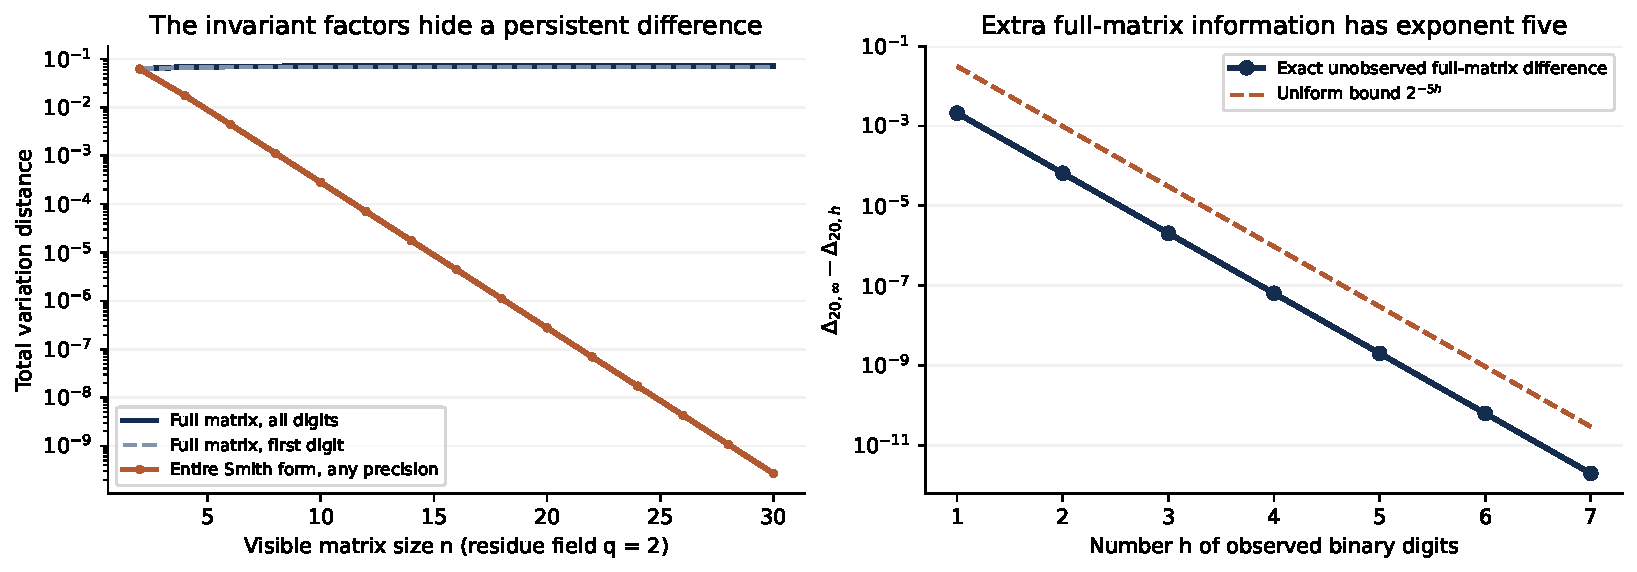
\includegraphics[width=.96\linewidth]{figures/precision_separation.pdf}
 \caption{Separation between the full-matrix and Smith-form laws,
 computed from the exact formulas. The full-matrix precision error
 obeys the sharp fifth-power law, whereas the Smith testing distance
 is independent of precision.}
 \label{fig:local-separation}
\end{figure}

The theorem therefore identifies both the information retained and the
information discarded by Smith normal form: the invariant factors
retain the entire module structure, while the alternating form on the
successive kernel modules carries an additional persistent constraint.


\clearpage
\section{Optimal graph couplings for zero transport}
\label{sec:graph-minimax}

The final question of the Article's section \texttt{zer:sec:open} asks which
graph minimizes the largest displacement bound in its electrical zero-transport
theorem, subject to a conductance budget and prescribed input degrees.
We solve this optimization, and its analogue for every Wasserstein distance
$W_p$, $1\le p\le\infty$. The result is unconditional finite-dimensional
mathematics. Dirichlet GRH supplies an application to finite packets of zero
ordinates.

\subsection{The optimization problem and its solution}

Fix $n\ge2$, integers $d_1,\ldots,d_n\ge1$, and a budget $W>0$. Put
\begin{equation}\label{gm:eq:C}
 N=\sum_{i=1}^n d_i,\qquad d=(d_i)_{i=1}^n,\qquad
 C=\operatorname{diag}(d_1,\ldots,d_n)-\frac{dd^{\mathsf T}}N.
\end{equation}
An admissible graph has these $n$ labelled vertices, conductances
$w_{ij}=w_{ji}\ge0$, connected positive support, and
$\sum_{i<j}w_{ij}=W$. Its Laplacian $L$ is positive definite on
$H=\mathbf1_n^\perp$ and has trace $2W$. The topology is free.

At vertex $i$ place a monic real-rooted polynomial $P_i$ of degree $d_i$.
Define
\begin{equation}\label{gm:eq:forest}
 \mathcal F_G(z)=\sum_{F}
 \left(\prod_{e\in F}w_e\right)
 \left(\prod_{i\in\mathcal R(F)}P_i'(z)\right)
 \left(\prod_{i\notin\mathcal R(F)}P_i(z)\right),
\end{equation}
where the sum is over spanning forests with one selected root in each
component and $\mathcal R(F)$ is the set of selected roots. There are $N-1$
real zeros $\lambda_1\le\cdots\le\lambda_{N-1}$ of this polynomial, counted
with multiplicity; a proof is given below. Let
$\beta_1\le\cdots\le\beta_{N-1}$ be the zeros of
$(\prod_iP_i)'$. Form the two empirical probability measures with mass
$1/(N-1)$ at each listed zero. Their one-dimensional Wasserstein distances are
\begin{align}
 W_p(\lambda,\beta)&=
 \left(\frac1{N-1}\sum_{k=1}^{N-1}|\beta_k-\lambda_k|^p\right)^{1/p}
 &&(1\le p<\infty),\label{gm:eq:Wp}\\
 W_\infty(\lambda,\beta)&=\max_k|\beta_k-\lambda_k|.\nonumber
\end{align}
Write $\mathcal E_p(G)$ for the supremum of this distance over all permitted
inputs $P_i$. This is a guarantee based only on their degrees, before their
roots are specified.

\begin{theorem}[Exact minimax graph]\label{gm:thm:main}
For $1\le p<\infty$, set $r=p/(p+1)$ and $S_r=\operatorname{tr}(C^r)$,
with the zero eigenvalue contributing zero. The unique optimal graph has
Laplacian
\begin{equation}\label{gm:eq:optimalL}
 L_p=\frac{2W}{S_r}C^r,
 \qquad
 \min_G\mathcal E_p(G)=
 \frac{S_r^{\,1+1/p}}{2W(N-1)^{1/p}}.
\end{equation}
For the largest displacement, the unique optimum is
\begin{align}
 L_\infty&=\frac{2W}{\operatorname{tr}C}C,
 &w_{ij}^{(\infty)}&=
 \frac{W d_i d_j}{\sum_{a<b}d_a d_b},\label{gm:eq:infinity}\\
 \min_G\mathcal E_\infty(G)&=
 \frac{\operatorname{tr}C}{2W}
 =\frac{N^2-\sum_i d_i^2}{2WN}.\nonumber
\end{align}
Every optimizer is a complete graph with strictly positive conductances.
For each fixed admissible graph, placing every input root at one common real
number attains its supremum. If all input roots are instead required to be
distinct, the supremum and the unique optimal graph are unchanged.
\end{theorem}

At $p=1$ the displacement is independent of the input roots, so no supremum
is needed. For $p>1$ we give an attaining configuration, without claiming that
it is the only attaining configuration. The normalization by $N-1$ in
\eqref{gm:eq:Wp} is essential: the perturbation has rank $n-1$, but there are
$N-1$ output zeros.

\subsection{The compression identity}

We first verify the finite identity behind the Article's electrical theorem.
List all input roots, repeated with their multiplicities and grouped by
vertex, as the diagonal entries of a real matrix $\Lambda$ of size $N$.
Let $V$ be the $N$ by $n$ matrix whose row for a root at vertex $i$ is $e_i^{\mathsf T}$.
Set
\begin{equation}\label{gm:eq:compression-data}
 Q=I_N-\frac{\mathbf1_N\mathbf1_N^{\mathsf T}}N,\quad
 \mathcal V=\mathbf1_N^\perp,\quad
 A=(Q\Lambda Q)|_{\mathcal V},\quad
 B=(QVL^+V^{\mathsf T}Q)|_{\mathcal V},
\end{equation}
where $L^+$ is the Moore--Penrose inverse.

\begin{lemma}[Forest compression]\label{gm:lem:compression}
If $\tau(G)$ is the sum of the conductance products of spanning trees, then
\[
 \mathcal F_G(z)=N\tau(G)\det_{\mathcal V}(zI-A+B),\qquad
 \left(\prod_iP_i(z)\right)'=N\det_{\mathcal V}(zI-A).
\]
Moreover, $B$ is positive semidefinite of rank $n-1$, and its nonzero
eigenvalues are the eigenvalues on $H$ of
\begin{equation}\label{gm:eq:reducedB}
 T_L=C^{1/2}(L|_H)^{-1}C^{1/2}.
\end{equation}
\end{lemma}

\begin{proof}
The matrix-tree theorem, applied after adding one extra vertex with edge
weights $x_i$ to the original vertices, gives the rooted-forest identity
\[
 \det(L+\operatorname{diag}(x_i))
 =\sum_F\left(\prod_{e\in F}w_e\right)
              \prod_{i\in\mathcal R(F)}x_i.
\]
Off the input roots, put $x_i=P_i'/P_i$ and multiply by
$P=\prod_iP_i$. Since
$V^{\mathsf T}(zI-\Lambda)^{-1}V=\operatorname{diag}(P_i'/P_i)$,
the Schur determinant formula gives
\[
 \mathcal F_G(z)=
 \det\begin{pmatrix}zI_N-\Lambda&V\\-V^{\mathsf T}&L\end{pmatrix}.
\]
Both sides are polynomials, so this identity holds everywhere.

Diagonalize $L$ in a basis beginning with
$u=\mathbf1_n/\sqrt n$ and eliminate its positive eigenvalue block.
The product of those eigenvalues is $n\tau(G)$, leaving the bordered
determinant with upper block
$zI_N-\Lambda+VL^+V^{\mathsf T}$ and border
$Vu=\mathbf1_N/\sqrt n$. For any nonzero real vector $b$ and any square
matrix $M$,
\[
 \det\begin{pmatrix}M&b\\-b^{\mathsf T}&0\end{pmatrix}
 =\|b\|^2\det_{b^\perp}(P_{b^\perp}M|_{b^\perp});
\]
expansion in an orthonormal basis ending with $b/\|b\|$ proves this.
Here $\|Vu\|^2=N/n$, proving the first identity.
The second follows from the cofactor identity
\[
 \det_{\mathcal V}(zI-A)
 =P(z)\frac1N\mathbf1_N^{\mathsf T}(zI-\Lambda)^{-1}\mathbf1_N
 =\frac{P'(z)}N.
\]

Finally, $V^{\mathsf T}QV=C$. The equal nonzero spectra of
$XX^{\mathsf T}$ and $X^{\mathsf T}X$, with
$X=QV(L^+)^{1/2}$, identify the positive spectrum of $B$ with that of
$T_L$. The quadratic identity
\[
 y^{\mathsf T}Cy=\frac1N\sum_{i<j}d_id_j(y_i-y_j)^2
\]
shows that $C$ is positive definite on $H$, proving the rank claim.
\end{proof}

In particular the output roots are real. Min--max gives
$\lambda_k\le\beta_k$ for all $k$.

\subsection{An exact worst-case envelope}

The eigenvalue perturbation inequality used next is classical Lidskii
majorization; see, for example, \cite[Theorem~2.1]{argentati2008}.
We include a proof of the specific convex-cost form required here.

\begin{lemma}[Convex displacement bound]\label{gm:lem:convex}
Let $A$ be real symmetric and $B\succeq0$ of the same size $m$.
Write ordered eigenvalues increasingly and let
$\Delta_k=\lambda_k(A)-\lambda_k(A-B)\ge0$.
For every continuous convex $\phi:[0,\infty)\to\mathbb R$,
\[
 \sum_{k=1}^m\phi(\Delta_k)\le\operatorname{tr}\phi(B).
\]
Equality holds for $A=cI$; for $\phi(t)=t$ it holds for every $A$.
\end{lemma}

\begin{proof}
First suppose $A$ has simple spectrum. The discriminant of the characteristic
polynomial of $A-tB$ is a polynomial in $t$ that is nonzero at zero, so only
finitely many $t\in[0,1]$ have repeated eigenvalues. At the other points,
\[
 -\lambda_k'(t)=u_k(t)^{\mathsf T}Bu_k(t)=b_k(t)\ge0
\]
for an orthonormal eigenbasis $u_k(t)$. The ordered eigenvalues are Lipschitz,
so $\Delta_k=\int_0^1b_k(t)\,dt$. Jensen's inequality gives
$\phi(\Delta_k)\le\int_0^1\phi(b_k(t))\,dt$.
In a $B$-eigenbasis, each $b_k(t)$ is a convex combination of its eigenvalues,
with weights equal to squared entries of an orthogonal matrix. A second
application of Jensen, summed over $k$, gives
$\sum_k\phi(b_k(t))\le\operatorname{tr}\phi(B)$.
Integrate. Approximation by matrices with simple spectrum proves the general
case. The two equality assertions follow directly from the spectra or the
trace identity.
\end{proof}

Apply this lemma with $\phi(t)=t^p$, and apply min--max for $p=\infty$.
The choice $P_i(z)=(z-c)^{d_i}$ makes $A=cI$ and attains the bound.
Together with Lemma~\ref{gm:lem:compression}, this proves the exact identities
\begin{equation}\label{gm:eq:exact-objective}
 \mathcal E_p(G)^p=\frac{\operatorname{tr}_H(T_L^p)}{N-1}
 \quad(1\le p<\infty),\qquad
 \mathcal E_\infty(G)=\|T_L\|.
\end{equation}
Arbitrarily small distinct perturbations of a common root give the same
supremum under the distinct-root restriction, by continuity of eigenvalues.

\subsection{Optimization, uniqueness, and graph feasibility}

\begin{proof}[Proof of Theorem~\ref{gm:thm:main}]
Work on $H$ in an orthonormal $C$-eigenbasis, with eigenvalues
$c_1,\ldots,c_{n-1}>0$. Put $\ell_i=L_{ii}>0$, so
$\sum_i\ell_i=2W$. For finite $p\ge1$, spectral Jensen and Cauchy--Schwarz give
\begin{align*}
 \operatorname{tr}(T_L^p)
 &\ge\sum_i ((T_L)_{ii})^p
 =\sum_i\bigl(c_i(L^{-1})_{ii}\bigr)^p
 \ge\sum_i(c_i/\ell_i)^p\\
 &\ge\frac{(\sum_i c_i^{p/(p+1)})^{p+1}}{(2W)^p}.
\end{align*}
Here $(L^{-1})_{ii}\ell_i\ge1$ is Cauchy--Schwarz for
$L^{1/2}e_i$ and $L^{-1/2}e_i$; equality forces $e_i$ to be an
$L$-eigenvector. The last inequality is the scalar constrained minimum of
$\sum_i c_i^p\ell_i^{-p}$, a strictly convex function: its unique minimizer is
$\ell_i=2Wc_i^{p/(p+1)}/S_r$.
Equality throughout therefore forces $L=(2W/S_r)C^r$.
This argument includes $p=1$: its first inequality is equality, but the inverse
diagonal inequality still forces diagonality and the scalar minimum is still
unique.

For $p=\infty$, let $t=\|T_L\|$. The inequality $T_L\preceq tI$
is equivalent to $C\preceq tL$. Thus
$t\ge\operatorname{tr}C/(2W)$. At equality $tL-C$ is positive semidefinite
with zero trace and is zero, giving the unique candidate in
\eqref{gm:eq:infinity}.

These lower bounds hold for all positive definite $L|_H$ of the prescribed
trace, even without the sign restrictions of a graph Laplacian. It remains
to verify that the candidates are graphs. For $0<r<1$, the scalar beta
integral and spectral calculus give
\[
 C^r=\frac{\sin(\pi r)}\pi\int_0^\infty
 t^{r-1}C(C+tI)^{-1}\,dt.
\]
This matrix annihilates $\mathbf1_n$. For $i\ne j$, the rank-one inverse
formula applied to $C+tI=\operatorname{diag}(d_i+t)-dd^{\mathsf T}/N$ gives
\[
 ((C+tI)^{-1})_{ij}=
 \frac{[d_i/(t+d_i)][d_j/(t+d_j)]}
 {t\sum_\ell d_\ell/(t+d_\ell)}>0.
\]
Consequently
\begin{equation}\label{gm:eq:edge-integral}
 -(C^r)_{ij}=\frac{\sin(\pi r)}\pi
 \int_0^\infty
 \frac{t^{r-1}d_id_j}
 {(t+d_i)(t+d_j)\sum_\ell d_\ell/(t+d_\ell)}\,dt>0.
\end{equation}
The integrand is $O(t^{r-1})$ at zero and $O(t^{r-2})$ at infinity.
Thus $C^r$ has strictly negative off-diagonal entries and is a connected
complete-graph Laplacian. At $r=1$ this follows from
$C_{ij}=-d_id_j/N$. Scaling gives trace $2W$ and the required budget.
Equation~\eqref{gm:eq:exact-objective} now gives the stated minima.
\end{proof}

Fractional powers of graph Laplacians are established objects;
\cite[Theorem~3.1]{benzi2022} gives a general preservation theorem.
Formula~\eqref{gm:eq:edge-integral} proves feasibility here directly and
provides an explicit positive integral for every optimal edge weight.

\begin{corollary}[Dependence on the displacement cost]\label{gm:cor:different}
If $n\ge3$, two distinct exponents $p\in[1,\infty]$ yield the same optimal
graph exactly when $d_1=\cdots=d_n$. In that case every optimal edge has
conductance $2W/[n(n-1)]$. For $n=2$ all exponents give the sole available
edge, of conductance $W$.
\end{corollary}

\begin{proof}
Equality of two normalized powers of $C$ with different exponents forces all
its positive eigenvalues to coincide. Thus $C=c(I_n-\mathbf1_n\mathbf1_n^{\mathsf T}/n)$.
Its off-diagonal entries imply that all products $d_id_j$ for $i\ne j$ are
equal; for $n\ge3$ this is equivalent to equal degrees. The converse and the
two-vertex case follow immediately.
\end{proof}

\subsection{An exact certificate for near-optimal mean transport}

\begin{proposition}[Mean-error gap and stability]\label{gm:prop:stability}
Let $L_*=L_1$, let $L$ be any admissible Laplacian, and set
$\Delta=L-L_*$ and $\delta=\mathcal E_1(L)/\mathcal E_1(L_*)-1$.
Then
\begin{equation}\label{gm:eq:gap}
 \delta=\frac1{2W}\operatorname{tr}(\Delta L^+\Delta),\qquad
 \|L-L_*\|_{\mathrm F}\le2W\sqrt\delta.
\end{equation}
For $n\ge3$, the exponent $1/2$ cannot be improved in a local bound uniform
over admissible Laplacians.
\end{proposition}

\begin{proof}
All inverses in this proof act on $H$. Write
$\alpha=2W/\operatorname{tr}\sqrt C$, so $C=L_*^2/\alpha^2$.
The exact resolvent identity is
\[
 L^{-1}=L_*^{-1}-L_*^{-1}\Delta L_*^{-1}
       +L_*^{-1}\Delta L^{-1}\Delta L_*^{-1}.
\]
Multiply by $C$ and take traces. Since $\operatorname{tr}\Delta=0$,
\[
 \operatorname{tr}(CL^{-1})-\operatorname{tr}(CL_*^{-1})
 =\alpha^{-2}\operatorname{tr}(\Delta L^{-1}\Delta),\qquad
 \operatorname{tr}(CL_*^{-1})=2W/\alpha^2.
\]
Equation~\eqref{gm:eq:exact-objective} proves the first claim.
Since $\lambda_{\max}(L)\le\operatorname{tr}L=2W$, the trace on the
right is at least $\|\Delta\|_{\mathrm F}^2/(2W)$.
For sharpness of the exponent, exchange a small amount of conductance
between two edges of the strictly positive optimal complete graph. This is
$L(t)=L_*+tK$ for nonzero symmetric $K$ with $K\mathbf1_n=0$
and $\operatorname{tr}K=0$. The exact formula gives
$\delta(t)=t^2\operatorname{tr}(K L_*^+K)/(2W)+O(t^3)$ with positive
quadratic coefficient, whereas $\|L(t)-L_*\|_{\mathrm F}=|t|\|K\|_{\mathrm F}$.
\end{proof}

\subsection{Unequal degrees: average and worst displacement disagree}

Take $(d_1,d_2,d_3)=(1,1,2)$ and $W=1$. The positive eigenvalues of $C$
are $1$ and $3/2$, with eigenvectors $(1,-1,0)$ and $(1,1,-2)$.
For $r=p/(p+1)$ and $s=(3/2)^r$, formula~\eqref{gm:eq:optimalL} gives
\[
 w_{12}=\frac{3-s}{3(1+s)},\qquad
 w_{13}=w_{23}=\frac{2s}{3(1+s)}.
\]
At $p=\infty$ these are $(1/5,2/5,2/5)$ and the optimal maximum
displacement is $5/4$. At $p=1$, $s=\sqrt6/2$, the edges are
\[
 \left(-3+\frac{4\sqrt6}3,\quad
 2-\frac{2\sqrt6}3,\quad 2-\frac{2\sqrt6}3\right),
\]
and the optimal mean displacement is $(5+2\sqrt6)/12$.
The graph optimal for the maximum has mean $5/6$, strictly larger than
$(5+2\sqrt6)/12$; the graph optimal for the mean has maximum
$(3+\sqrt6)/4$, strictly larger than $5/4$.

For the attaining inputs $(P_1,P_2,P_3)=(z,z,z^2)$ and conductances
$(w_{12},w_{13},w_{23})=(x,y,y)$, direct expansion gives
\[
 \mathcal F_G(z)=2z+(4x+6y)z^2+4(2xy+y^2)z^3.
\]
At the maximum-optimal graph this factors as
$\frac{32}{25}z(z+\frac54)^2$, whereas $(P_1P_2P_3)'=4z^3$.
At the mean-optimal graph the displacement multiset is
$\{0,(1+s)/2,s(1+s)/2\}$.

The supplied verifier checks these identities symbolically, an exact
noncollapsed forest/compression example, and the stability certificate.
Its numerical diagnostics also check $75$ optimal configurations,
$750$ competing graphs and $150$ checks comparing noncollapsed inputs
with the collapsed extremizer. Those diagnostics check implementation and constants;
the theorem rests on the proof above.

\subsection{Application to finite Dirichlet-zero packets}

Under the Dirichlet GRH theorem in the vendored development, the phase-normalized
completed primitive Dirichlet $L$-functions have real ordinate zeros. Select a
finite packet of $d_i$ such zeros at vertex $i$, preserving the selected
multiplicities, and make $P_i$ their monic root polynomial. Theorem~\ref{gm:thm:main}
gives the best uniform guarantee based only on the packet sizes and budget.
It allows shared zeros, multiple zeros and arbitrary spacings.
A particular arithmetic packet may admit a smaller error and a different
optimal graph; the common-root extremizer need not occur for Dirichlet
functions. No optimum for an entire infinite zero set is inferred.

\clearpage
\section{Verification, reproducibility, and formalization}
\label{sec:verification}

\subsection{Exact checks and numerical diagnostics}

The proofs in this paper are human-readable mathematical arguments. The
finite computations below check their counting formulas, normalizations,
equality cases, and constants. They do not replace the proofs. All finite-ring
enumerations and probability comparisons use integers or exact rational
arithmetic; the graph example also uses exact symbolic algebra.

\begin{center}
\small
\begin{tabular}{>{\raggedright\arraybackslash}p{0.30\linewidth}>{\raggedright\arraybackslash}p{0.61\linewidth}}
\hline
Check & Verified extent and outcome\\
\hline
Binary symplectic fibers &
All $65{,}536$ matrices in $\operatorname{Mat}_4(\mathbb F_2)$ were checked
against their linear Gram-equation fibers. Exactly $61{,}110$ matrices
were supported; the fiber sum was $65{,}802{,}240$.\\[3pt]
Small-ring pairs &
All $65{,}536$ pairs of $2\times2$ matrices over $\mathbb Z/4\mathbb Z$
and all $6{,}561$ pairs over $\mathbb F_3$ were enumerated.
The Smith distances were exactly $1/16$ and $1/81$.\\[3pt]
Deep Smith orientations &
All $4{,}096$ alternating $4\times4$ forms over $\mathbb Z/4\mathbb Z$
were enumerated. All $15$ capped Smith types agreed with their predicted
support probabilities among the $1{,}792$ unimodular forms.\\[3pt]
Probability identities &
$70$ pairs $(q,n)$, with $q\in\{2,3,4,5,7,8,9\}$ and
$n\in\{2,4,\ldots,20\}$, passed exact normalization, Smith-distance,
and monotonicity checks.\\[3pt]
Graph certificates &
$11$ symbolic checks verified the unequal-degree example, forest
identities, optimal costs, and the mean-error stability certificate.\\
\hline
\end{tabular}
\end{center}

The records are \texttt{results/exact\_verification.json} and
\texttt{results/graph\_verification.json}. Separate floating-point graph
diagnostics covered $75$ optimizers, $750$ competitor comparisons, and
$150$ checks comparing noncollapsed inputs with the collapsed extremizer. An independently
written diagnostic checked a further $2{,}000$ graph comparisons across
$50$ degree profiles. These numerical runs support implementation checks;
their tolerances are not interval certificates or kernel proofs.

The limiting constants are different: their enclosing endpoints are exact
rational numbers obtained from finite products, finite recurrences, and a
proved series-tail estimate. The printed decimals and figures are rounded
displays of those certificates. The endpoints and finite values are retained
in \texttt{results/tables\_and\_certificates.json}.

\subsection{Reproducing the artifacts}

Run the following commands from the extracted archive directory:
\begin{verbatim}
python3 code/verify_exact.py
python3 code/make_tables.py
python3 code/verify_graph_minimax.py \
  --output results/graph_verification.json
python3 code/independent_graph_check.py
pdflatex -interaction=nonstopmode -halt-on-error paper.tex
pdflatex -interaction=nonstopmode -halt-on-error paper.tex
\end{verbatim}
The exact symplectic verifier uses only the Python standard library.
The graph verifier uses NumPy and SymPy; the independent graph diagnostic
uses NumPy. The tables use the standard library, with Matplotlib needed
to regenerate the figure. The PDF uses ordinary LaTeX packages and an
included bibliography, so no bibliography download or BibTeX run is needed.

\subsection{Source map}

Both requested source directories were read at ProveIt commit
\begin{center}\small\sourcecommit.\end{center}
The vendored Lean development identifies its upstream revision as
\begin{center}\small\upstreamcommit.\end{center}
Full source URLs and
the distinction between inherited results and new arguments are recorded
in \texttt{PROVENANCE.txt}.

The direct mathematical starting points in the Article are
\texttt{sections/spn.tex}, labels \texttt{spn:thm:lagrangian} and
\texttt{spn:thm:rank-blind}, for the finite-field projection laws, and
\texttt{sections/zer.tex}, label \texttt{zer:thm:electrical}, for graph
zero transport. The last question of \texttt{zer:sec:open} is the
largest-displacement optimization solved here.

Within the vendored package, \texttt{src/Statements.lean} fixes the public
RH and Dirichlet-GRH predicates in Mathlib terms, and
\texttt{src/Main.lean} connects them to the proof. The files
\nolinkurl{src/New/Reduction/MainInequality.lean},
\nolinkurl{src/New/Reduction/OneSidedBound.lean}, and
\nolinkurl{src/New/Reduction/Zeros/Criterion.lean} locate, respectively,
the covolume comparison, the one-sided arithmetic estimate, and the
analytic passage to nonvanishing. This paper inspects those source
connections; it does not claim to have rebuilt the entire upstream proof.

\subsection{Formalization status and scope}

No new theorem in this paper is presented as Lean-checked. The accompanying
\texttt{FORMALIZATION.txt} gives a dependency-oriented implementation plan,
beginning with the finite-ring Gram fibers and the finite-dimensional graph
optimization. Copies of upstream Lean files, when included for provenance,
are source inputs, not formalizations of the new theorems.

The local random-matrix result is unconditional. Its connection to the
requested material is a mathematical extension of the Article's
finite-field compression method. The graph optimization is also
unconditional; its application to finite Dirichlet-zero packets uses the
upstream Dirichlet-GRH theorem. No infinite-zero-set minimax claim or
new Artin or automorphic GRH theorem is made. The comparison with the
Article establishes a distinct extension of that collection. The
literature checks described in this paper do not certify worldwide
priority.

\clearpage
\phantomsection
\addcontentsline{toc}{section}{References}
\begin{thebibliography}{99}

\bibitem{ProveItArticle}
ProveIt Contributors.
\emph{Beyond the Riemann hypothesis for Dirichlet \(L\)-functions:
consequences, transfers and limits}.
Merged article, 26 November 2026.
Inspected at revision \texttt{3d8689ceae76}.
\href{https://github.com/VladimirReshetnikov/ProveIt/tree/3d8689ceae76501a5c50f67da37e85369aac4fb6/Analysis/GeneralizedRiemannHypothesis/Article}{Pinned article directory}.
Relevant sources:
\href{https://github.com/VladimirReshetnikov/ProveIt/blob/3d8689ceae76501a5c50f67da37e85369aac4fb6/Analysis/GeneralizedRiemannHypothesis/Article/sections/spn.tex}{\texttt{sections/spn.tex}} and
\href{https://github.com/VladimirReshetnikov/ProveIt/blob/3d8689ceae76501a5c50f67da37e85369aac4fb6/Analysis/GeneralizedRiemannHypothesis/Article/sections/zer.tex}{\texttt{sections/zer.tex}}.

\bibitem{ProveItVendor}
ProveIt Contributors.
\emph{Vendored grh-lean (readable edition)}.
\href{https://github.com/VladimirReshetnikov/ProveIt/blob/3d8689ceae76501a5c50f67da37e85369aac4fb6/Analysis/GeneralizedRiemannHypothesis/vendor/grh-lean/README.md}{Pinned vendor README}, 27 November 2026.

\bibitem{SourceStatements}
\texttt{lsernau/grh-lean}.
\emph{Statements and public theorem endpoints}.
Readable package at upstream revision \texttt{72fead102f66},
vendored without alteration in ProveIt.
\href{https://github.com/VladimirReshetnikov/ProveIt/blob/3d8689ceae76501a5c50f67da37e85369aac4fb6/Analysis/GeneralizedRiemannHypothesis/vendor/grh-lean/grh/src/Statements.lean}{\texttt{src/Statements.lean}} and
\href{https://github.com/VladimirReshetnikov/ProveIt/blob/3d8689ceae76501a5c50f67da37e85369aac4fb6/Analysis/GeneralizedRiemannHypothesis/vendor/grh-lean/grh/src/Main.lean}{\texttt{src/Main.lean}}.

\bibitem{SourceReadme}
\texttt{lsernau/grh-lean}.
\emph{Readable package README and axiom-check commands}.
\href{https://github.com/VladimirReshetnikov/ProveIt/blob/3d8689ceae76501a5c50f67da37e85369aac4fb6/Analysis/GeneralizedRiemannHypothesis/vendor/grh-lean/grh/README.md}{Pinned upstream README}.
The build/checker claims summarized in this report are the source's reports;
they were not replayed here.

\bibitem{SourceCriterion}
\texttt{lsernau/grh-lean}.
\emph{One-sided zero criterion}.
\href{https://github.com/VladimirReshetnikov/ProveIt/blob/3d8689ceae76501a5c50f67da37e85369aac4fb6/Analysis/GeneralizedRiemannHypothesis/vendor/grh-lean/grh/src/New/Reduction/Zeros/Criterion.lean}{\texttt{New/Reduction/Zeros/Criterion.lean}}.
See also the saved source subset's \texttt{Lib/Analytic/Landau.lean}.

\bibitem{SourceInequality}
\texttt{lsernau/grh-lean}.
\emph{Main covolume inequality}.
\href{https://github.com/VladimirReshetnikov/ProveIt/blob/3d8689ceae76501a5c50f67da37e85369aac4fb6/Analysis/GeneralizedRiemannHypothesis/vendor/grh-lean/grh/src/New/Reduction/MainInequality.lean}{\texttt{New/Reduction/MainInequality.lean}}.

\bibitem{SourceOneSided}
\texttt{lsernau/grh-lean}.
\emph{One-sided prime-remainder bound}.
\href{https://github.com/VladimirReshetnikov/ProveIt/blob/3d8689ceae76501a5c50f67da37e85369aac4fb6/Analysis/GeneralizedRiemannHypothesis/vendor/grh-lean/grh/src/New/Reduction/OneSidedBound.lean}{\texttt{New/Reduction/OneSidedBound.lean}}.

\bibitem{FulmanGoldstein}
J. Fulman and L. Goldstein.
Stein's method and the rank distribution of random matrices over finite fields.
\emph{Annals of Probability} \textbf{43}(3) (2015), 1274--1314.
\href{https://doi.org/10.1214/13-AOP889}{doi:10.1214/13-AOP889}.
\href{https://arxiv.org/abs/1211.0504}{arXiv:1211.0504}.

\bibitem{WangStanley}
Y. Wang and R. P. Stanley.
The Smith normal form distribution of a random integer matrix.
\emph{SIAM Journal on Discrete Mathematics} \textbf{31}(3) (2017), 2247--2268.
\href{https://doi.org/10.1137/16M1098140}{doi:10.1137/16M1098140}.
\href{https://math.mit.edu/~rstan/papers/randomsnf.pdf}{Author manuscript}.

\bibitem{VanPeski2021}
R. Van Peski.
Limits and fluctuations of \(p\)-adic random matrix products.
\emph{Selecta Mathematica} \textbf{27} (2021), article 98.
\href{https://doi.org/10.1007/s00029-021-00709-3}{doi:10.1007/s00029-021-00709-3}.
\href{https://arxiv.org/abs/2011.09356}{arXiv:2011.09356}.

\bibitem{VanPeski2024}
R. Van Peski.
Local limits in \(p\)-adic random matrix theory.
\emph{Proceedings of the London Mathematical Society} \textbf{129} (2024), e12626.
\href{https://doi.org/10.1112/plms.12626}{doi:10.1112/plms.12626}.
\href{https://arxiv.org/abs/2310.12275}{arXiv:2310.12275}.

\bibitem{GhoshBoydSaberi}
A. Ghosh, S. Boyd, and A. Saberi.
Minimizing effective resistance of a graph.
\emph{SIAM Review} \textbf{50}(1) (2008), 37--66.
\href{https://doi.org/10.1137/050645452}{doi:10.1137/050645452}.
\href{https://web.stanford.edu/~boyd/papers/pdf/eff_res.pdf}{Author PDF}.

\bibitem{benzi2022}
M. Benzi and I. Simunec.
Rational Krylov methods for fractional diffusion problems on graphs.
\emph{BIT Numerical Mathematics} \textbf{62} (2022), 357--385.
\href{https://doi.org/10.1007/s10543-021-00881-0}{doi:10.1007/s10543-021-00881-0}.

\bibitem{argentati2008}
M. E. Argentati, A. V. Knyazev, C. C. Paige, and I. Panayotov.
Bounds on changes in Ritz values for a perturbed invariant subspace of a
Hermitian matrix. 2008 manuscript, Theorem 2.1.
\href{https://arxiv.org/abs/math/0610498}{arXiv:math/0610498}.
\href{https://www.cs.mcgill.ca/~chris/pub/ArgKPP08.pdf}{Author PDF}.
\end{thebibliography}

\end{document}
